\documentclass[]{article}
\usepackage{lmodern}
\usepackage{amssymb,amsmath}
\usepackage{ifxetex,ifluatex}
\usepackage{fixltx2e} % provides \textsubscript
\ifnum 0\ifxetex 1\fi\ifluatex 1\fi=0 % if pdftex
  \usepackage[T1]{fontenc}
  \usepackage[utf8]{inputenc}
\else % if luatex or xelatex
  \ifxetex
    \usepackage{mathspec}
  \else
    \usepackage{fontspec}
  \fi
  \defaultfontfeatures{Ligatures=TeX,Scale=MatchLowercase}
\fi
% use upquote if available, for straight quotes in verbatim environments
\IfFileExists{upquote.sty}{\usepackage{upquote}}{}
% use microtype if available
\IfFileExists{microtype.sty}{%
\usepackage{microtype}
\UseMicrotypeSet[protrusion]{basicmath} % disable protrusion for tt fonts
}{}
\usepackage[margin=1in]{geometry}
\usepackage{hyperref}
\hypersetup{unicode=true,
            pdftitle={Fan Ratings},
            pdfauthor={Steven Miller},
            pdfborder={0 0 0},
            breaklinks=true}
\urlstyle{same}  % don't use monospace font for urls
\usepackage{color}
\usepackage{fancyvrb}
\newcommand{\VerbBar}{|}
\newcommand{\VERB}{\Verb[commandchars=\\\{\}]}
\DefineVerbatimEnvironment{Highlighting}{Verbatim}{commandchars=\\\{\}}
% Add ',fontsize=\small' for more characters per line
\usepackage{framed}
\definecolor{shadecolor}{RGB}{248,248,248}
\newenvironment{Shaded}{\begin{snugshade}}{\end{snugshade}}
\newcommand{\KeywordTok}[1]{\textcolor[rgb]{0.13,0.29,0.53}{\textbf{#1}}}
\newcommand{\DataTypeTok}[1]{\textcolor[rgb]{0.13,0.29,0.53}{#1}}
\newcommand{\DecValTok}[1]{\textcolor[rgb]{0.00,0.00,0.81}{#1}}
\newcommand{\BaseNTok}[1]{\textcolor[rgb]{0.00,0.00,0.81}{#1}}
\newcommand{\FloatTok}[1]{\textcolor[rgb]{0.00,0.00,0.81}{#1}}
\newcommand{\ConstantTok}[1]{\textcolor[rgb]{0.00,0.00,0.00}{#1}}
\newcommand{\CharTok}[1]{\textcolor[rgb]{0.31,0.60,0.02}{#1}}
\newcommand{\SpecialCharTok}[1]{\textcolor[rgb]{0.00,0.00,0.00}{#1}}
\newcommand{\StringTok}[1]{\textcolor[rgb]{0.31,0.60,0.02}{#1}}
\newcommand{\VerbatimStringTok}[1]{\textcolor[rgb]{0.31,0.60,0.02}{#1}}
\newcommand{\SpecialStringTok}[1]{\textcolor[rgb]{0.31,0.60,0.02}{#1}}
\newcommand{\ImportTok}[1]{#1}
\newcommand{\CommentTok}[1]{\textcolor[rgb]{0.56,0.35,0.01}{\textit{#1}}}
\newcommand{\DocumentationTok}[1]{\textcolor[rgb]{0.56,0.35,0.01}{\textbf{\textit{#1}}}}
\newcommand{\AnnotationTok}[1]{\textcolor[rgb]{0.56,0.35,0.01}{\textbf{\textit{#1}}}}
\newcommand{\CommentVarTok}[1]{\textcolor[rgb]{0.56,0.35,0.01}{\textbf{\textit{#1}}}}
\newcommand{\OtherTok}[1]{\textcolor[rgb]{0.56,0.35,0.01}{#1}}
\newcommand{\FunctionTok}[1]{\textcolor[rgb]{0.00,0.00,0.00}{#1}}
\newcommand{\VariableTok}[1]{\textcolor[rgb]{0.00,0.00,0.00}{#1}}
\newcommand{\ControlFlowTok}[1]{\textcolor[rgb]{0.13,0.29,0.53}{\textbf{#1}}}
\newcommand{\OperatorTok}[1]{\textcolor[rgb]{0.81,0.36,0.00}{\textbf{#1}}}
\newcommand{\BuiltInTok}[1]{#1}
\newcommand{\ExtensionTok}[1]{#1}
\newcommand{\PreprocessorTok}[1]{\textcolor[rgb]{0.56,0.35,0.01}{\textit{#1}}}
\newcommand{\AttributeTok}[1]{\textcolor[rgb]{0.77,0.63,0.00}{#1}}
\newcommand{\RegionMarkerTok}[1]{#1}
\newcommand{\InformationTok}[1]{\textcolor[rgb]{0.56,0.35,0.01}{\textbf{\textit{#1}}}}
\newcommand{\WarningTok}[1]{\textcolor[rgb]{0.56,0.35,0.01}{\textbf{\textit{#1}}}}
\newcommand{\AlertTok}[1]{\textcolor[rgb]{0.94,0.16,0.16}{#1}}
\newcommand{\ErrorTok}[1]{\textcolor[rgb]{0.64,0.00,0.00}{\textbf{#1}}}
\newcommand{\NormalTok}[1]{#1}
\usepackage{graphicx,grffile}
\makeatletter
\def\maxwidth{\ifdim\Gin@nat@width>\linewidth\linewidth\else\Gin@nat@width\fi}
\def\maxheight{\ifdim\Gin@nat@height>\textheight\textheight\else\Gin@nat@height\fi}
\makeatother
% Scale images if necessary, so that they will not overflow the page
% margins by default, and it is still possible to overwrite the defaults
% using explicit options in \includegraphics[width, height, ...]{}
\setkeys{Gin}{width=\maxwidth,height=\maxheight,keepaspectratio}
\IfFileExists{parskip.sty}{%
\usepackage{parskip}
}{% else
\setlength{\parindent}{0pt}
\setlength{\parskip}{6pt plus 2pt minus 1pt}
}
\setlength{\emergencystretch}{3em}  % prevent overfull lines
\providecommand{\tightlist}{%
  \setlength{\itemsep}{0pt}\setlength{\parskip}{0pt}}
\setcounter{secnumdepth}{0}
% Redefines (sub)paragraphs to behave more like sections
\ifx\paragraph\undefined\else
\let\oldparagraph\paragraph
\renewcommand{\paragraph}[1]{\oldparagraph{#1}\mbox{}}
\fi
\ifx\subparagraph\undefined\else
\let\oldsubparagraph\subparagraph
\renewcommand{\subparagraph}[1]{\oldsubparagraph{#1}\mbox{}}
\fi

%%% Use protect on footnotes to avoid problems with footnotes in titles
\let\rmarkdownfootnote\footnote%
\def\footnote{\protect\rmarkdownfootnote}

%%% Change title format to be more compact
\usepackage{titling}

% Create subtitle command for use in maketitle
\providecommand{\subtitle}[1]{
  \posttitle{
    \begin{center}\large#1\end{center}
    }
}

\setlength{\droptitle}{-2em}

  \title{Fan Ratings}
    \pretitle{\vspace{\droptitle}\centering\huge}
  \posttitle{\par}
    \author{Steven Miller}
    \preauthor{\centering\large\emph}
  \postauthor{\par}
      \predate{\centering\large\emph}
  \postdate{\par}
    \date{April 6, 2019}


\begin{document}
\maketitle

\subsection{Fan Ratings Dataset}\label{fan-ratings-dataset}

\begin{Shaded}
\begin{Highlighting}[]
\NormalTok{ratings <-}\StringTok{ }\KeywordTok{read.csv}\NormalTok{(}\StringTok{'data/fan_ratings.csv'}\NormalTok{)}
\end{Highlighting}
\end{Shaded}

Summary of Fan Ratings:

\begin{Shaded}
\begin{Highlighting}[]
\KeywordTok{summary}\NormalTok{(ratings)}
\end{Highlighting}
\end{Shaded}

\begin{verbatim}
##        Y              R                    GPNAME           P1    
##  Min.   :2008   Min.   : 1.000   Australian GP: 11   Hamilton:62  
##  1st Qu.:2010   1st Qu.: 5.000   Belgian GP   : 11   Vettel  :52  
##  Median :2013   Median :10.000   British GP   : 11   Rosberg :22  
##  Mean   :2013   Mean   : 9.822   Chinese GP   : 11   Button  :14  
##  3rd Qu.:2016   3rd Qu.:14.000   Hungarian GP : 11   Alonso  :13  
##  Max.   :2018   Max.   :21.000   Monaco GP    : 11   Webber  : 9  
##                                  (Other)      :136   (Other) :30  
##          P2             P3         RATING     
##  Hamilton :30   Raikkonen:26   Min.   :3.740  
##  Vettel   :29   Vettel   :26   1st Qu.:5.777  
##  Rosberg  :25   Hamilton :21   Median :6.812  
##  Alonso   :19   Alonso   :16   Mean   :6.793  
##  Raikkonen:19   Ricciardo:15   3rd Qu.:7.801  
##  Webber   :16   Webber   :15   Max.   :9.449  
##  (Other)  :64   (Other)  :83
\end{verbatim}

Y - Year of Race\\
R - Round of Race in Season\\
GPNAME - Name of Race\\
P1 - Race Winner\\
P2 - Runner-Up\\
P3 - Third Place\\
RATING - Average fan rating on a scale from 1 to 10

\begin{Shaded}
\begin{Highlighting}[]
\KeywordTok{ggplot}\NormalTok{(ratings, }\KeywordTok{aes}\NormalTok{(RATING)) }\OperatorTok{+}\StringTok{ }\KeywordTok{geom_histogram}\NormalTok{(}\KeywordTok{aes}\NormalTok{(}\DataTypeTok{y=}\NormalTok{..density..), }\DataTypeTok{binwidth =} \FloatTok{0.5}\NormalTok{) }\OperatorTok{+}\StringTok{ }
\StringTok{  }\KeywordTok{stat_function}\NormalTok{(}\DataTypeTok{fun =}\NormalTok{ dnorm, }\DataTypeTok{args =} \KeywordTok{list}\NormalTok{(}\DataTypeTok{mean =} \KeywordTok{mean}\NormalTok{(ratings}\OperatorTok{$}\NormalTok{RATING), }\DataTypeTok{sd =} \KeywordTok{sd}\NormalTok{(ratings}\OperatorTok{$}\NormalTok{RATING))) }\OperatorTok{+}\StringTok{ }
\StringTok{  }\KeywordTok{labs}\NormalTok{(}\DataTypeTok{title=}\StringTok{"Average Fan Rating of Grands Prix"}\NormalTok{, }\DataTypeTok{y=}\StringTok{"Density"}\NormalTok{, }\DataTypeTok{x=}\StringTok{"Rating"}\NormalTok{)}
\end{Highlighting}
\end{Shaded}

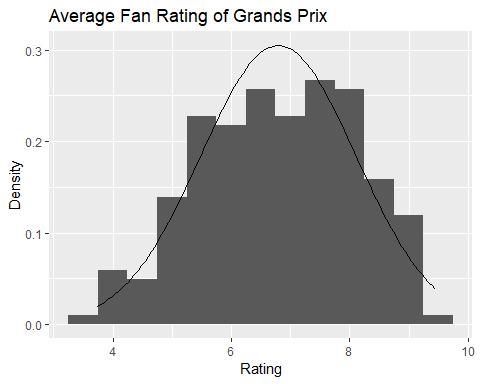
\includegraphics{part_1_files/figure-latex/unnamed-chunk-2-1.pdf}

Is it possible that certain drivers winning a race would have an impact
on the fan rating? It seems like a possibility to me. A fan of a certain
driver might be more likely to give a race a higher rating if they
enjoyed the race. Looking at the summary of the ratings table, it
appears that the five winningest drivers in the data set were Hamilton,
Vettel, Rosberg, Button, and Alonso. We also know that the mean rating
is 6.793. Let's see what the average rating is for races where these
drivers won.

\begin{Shaded}
\begin{Highlighting}[]
\NormalTok{agg <-}\StringTok{ }\KeywordTok{aggregate}\NormalTok{(ratings}\OperatorTok{$}\NormalTok{RATING, }\DataTypeTok{by =} \KeywordTok{list}\NormalTok{(ratings}\OperatorTok{$}\NormalTok{P1), }\DataTypeTok{FUN =}\NormalTok{ mean)}
\NormalTok{agg <-}\StringTok{ }\NormalTok{agg[}\KeywordTok{order}\NormalTok{(}\OperatorTok{-}\NormalTok{agg}\OperatorTok{$}\NormalTok{x),]}
\KeywordTok{names}\NormalTok{(agg) <-}\StringTok{ }\KeywordTok{c}\NormalTok{(}\StringTok{"Driver"}\NormalTok{,}\StringTok{"Rating"}\NormalTok{)}
\KeywordTok{print}\NormalTok{(agg)}
\end{Highlighting}
\end{Shaded}

\begin{verbatim}
##        Driver   Rating
## 8   Maldonado 8.274000
## 11  Ricciardo 8.108571
## 7      Kubica 7.809000
## 13 Verstappen 7.732500
## 4      Button 7.307286
## 10  Raikkonen 7.045400
## 5    Hamilton 6.945645
## 1      Alonso 6.799077
## 14     Vettel 6.569173
## 15     Webber 6.517000
## 12    Rosberg 6.449364
## 2  Barichello 6.202000
## 6  Kovalainen 6.202000
## 9       Massa 6.104333
## 3      Bottas 4.836667
\end{verbatim}

Recalling that our mean rating was 6.793 it appears that the five
winningest drivers are all pretty close to this mean. From this, one
could hypothesize that fans find it more or less exciting when a driver
who doesn't typically win races wins.

\subsection{Ergast F1 Dataset}\label{ergast-f1-dataset}

The first variable we'll take a look at is the duration of pit stops.
Throughout many seasons, the rules regarding pit stops have changed.
Over time, various seasons of racing will have had various average
durations for pit stops. This can be a matter of seconds but leads to
big changes in strategic decision making that can impact the way a race
plays out.

\begin{Shaded}
\begin{Highlighting}[]
\NormalTok{pitstops <-}\StringTok{ }\KeywordTok{read.csv}\NormalTok{(}\StringTok{'data/pit_stops.csv'}\NormalTok{, }\DataTypeTok{header=}\OtherTok{FALSE}\NormalTok{, }\DataTypeTok{col.names =} \KeywordTok{c}\NormalTok{(}\StringTok{"raceId"}\NormalTok{,}\StringTok{"driverId"}\NormalTok{,}\StringTok{"stop"}\NormalTok{,}\StringTok{"lap"}\NormalTok{,}\StringTok{"time"}\NormalTok{,}\StringTok{"duration"}\NormalTok{,}\StringTok{"milliseconds"}\NormalTok{))}
\KeywordTok{summary}\NormalTok{(pitstops)}
\end{Highlighting}
\end{Shaded}

\begin{verbatim}
##      raceId          driverId          stop            lap       
##  Min.   : 841.0   Min.   :  1.0   Min.   :1.000   Min.   : 1.00  
##  1st Qu.: 871.0   1st Qu.: 16.0   1st Qu.:1.000   1st Qu.:13.00  
##  Median : 909.0   Median :807.0   Median :2.000   Median :24.00  
##  Mean   : 915.9   Mean   :447.4   Mean   :1.793   Mean   :24.83  
##  3rd Qu.: 959.0   3rd Qu.:822.0   3rd Qu.:2.000   3rd Qu.:35.00  
##  Max.   :1011.0   Max.   :848.0   Max.   :6.000   Max.   :74.00  
##                                                                  
##        time         duration     milliseconds    
##  14:56:46:   5   22.303 :   6   Min.   :  12897  
##  14:05:02:   4   22.838 :   6   1st Qu.:  21811  
##  14:18:36:   4   21.012 :   5   Median :  23375  
##  14:19:03:   4   21.900 :   5   Mean   :  45738  
##  14:20:17:   4   22.105 :   5   3rd Qu.:  25567  
##  14:20:51:   4   22.273 :   5   Max.   :2011266  
##  (Other) :6824   (Other):6817
\end{verbatim}

\begin{Shaded}
\begin{Highlighting}[]
\KeywordTok{head}\NormalTok{(pitstops)}
\end{Highlighting}
\end{Shaded}

\begin{verbatim}
##   raceId driverId stop lap     time duration milliseconds
## 1    841      153    1   1 17:05:23   26.898        26898
## 2    841       30    1   1 17:05:52   25.021        25021
## 3    841       17    1  11 17:20:48   23.426        23426
## 4    841        4    1  12 17:22:34   23.251        23251
## 5    841       13    1  13 17:24:10   23.842        23842
## 6    841       22    1  13 17:24:29   23.643        23643
\end{verbatim}

raceId - the database id of the race the pit stop took place in driverId
- the database id of the driver making a pit stop stop - the stop number
out of all stops a driver made in a particular race lap - the lap number
the pit stop was conducted on time - the time of day the pit stop took
place duration - how long the pit stop took milliseconds - duration, but
in milliseconds

We can see from the summary that there are some vast outliers in the
milliseconds column. We have a max value of almost forty minutes and a
minimum value of 12.897 seconds. The mean is 45.738 and a median of
23.375. Based on these values, it's clear that the outliers are skewing
the data. With a little bit of domain knowledge, I can safely say that
any pit stops taking that long were not done by vehicles who were
actually competitive during the race and can pretty safely be excluded
from further analysis.

\begin{Shaded}
\begin{Highlighting}[]
\NormalTok{stopsd <-}\StringTok{ }\KeywordTok{sd}\NormalTok{(pitstops}\OperatorTok{$}\NormalTok{milliseconds)}
\KeywordTok{print}\NormalTok{(stopsd)}
\end{Highlighting}
\end{Shaded}

\begin{verbatim}
## [1] 171321.9
\end{verbatim}

Looking at the standard deviation of pit stop duration, it appears to be
171 milliseconds. I feel comfortable excluding any values greater than
one-half standard deviation over the mean from further analysis, as this
would indicate pit stops over two minutes in length.

\begin{Shaded}
\begin{Highlighting}[]
\NormalTok{pitstops <-}\StringTok{ }\NormalTok{pitstops[pitstops}\OperatorTok{$}\NormalTok{milliseconds}\OperatorTok{<=}\KeywordTok{mean}\NormalTok{(pitstops}\OperatorTok{$}\NormalTok{milliseconds)}\OperatorTok{+}\NormalTok{stopsd}\OperatorTok{/}\DecValTok{2}\NormalTok{,]}
\end{Highlighting}
\end{Shaded}

With those values removed from the data, we can now further analyze the
duration.

\begin{Shaded}
\begin{Highlighting}[]
\KeywordTok{ggplot}\NormalTok{(pitstops, }\KeywordTok{aes}\NormalTok{(milliseconds)) }\OperatorTok{+}\StringTok{ }\KeywordTok{geom_histogram}\NormalTok{(}\DataTypeTok{binwidth =} \DecValTok{60}\NormalTok{)}
\end{Highlighting}
\end{Shaded}

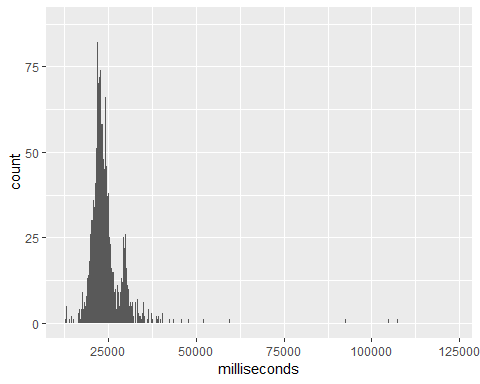
\includegraphics{part_1_files/figure-latex/unnamed-chunk-7-1.pdf}

We can now see the peak around 25 seconds as well as a second, smaller
spike around 30 seconds. This is likely due to rule changes at some
point that either sped up or slowed down the average pit stop duration.
It would be interesting, I think, to see how the average time has
changed over the years. If we combine some tables together we can look
into this further.

\subsection{F1 races table}\label{f1-races-table}

\begin{Shaded}
\begin{Highlighting}[]
\NormalTok{races <-}\StringTok{ }\KeywordTok{read.csv}\NormalTok{(}\StringTok{'data/races.csv'}\NormalTok{, }\DataTypeTok{header=}\OtherTok{FALSE}\NormalTok{, }\DataTypeTok{col.names=}\KeywordTok{c}\NormalTok{(}\StringTok{"raceId"}\NormalTok{,}\StringTok{"year"}\NormalTok{,}\StringTok{"round"}\NormalTok{,}\StringTok{"circuitId"}\NormalTok{,}\StringTok{"name"}\NormalTok{,}\StringTok{"date"}\NormalTok{,}\StringTok{"time"}\NormalTok{,}\StringTok{"url"}\NormalTok{))}
\KeywordTok{head}\NormalTok{(races)}
\end{Highlighting}
\end{Shaded}

\begin{verbatim}
##   raceId year round circuitId                  name       date     time
## 1      1 2009     1         1 Australian Grand Prix 2009-03-29 06:00:00
## 2      2 2009     2         2  Malaysian Grand Prix 2009-04-05 09:00:00
## 3      3 2009     3        17    Chinese Grand Prix 2009-04-19 07:00:00
## 4      4 2009     4         3    Bahrain Grand Prix 2009-04-26 12:00:00
## 5      5 2009     5         4    Spanish Grand Prix 2009-05-10 12:00:00
## 6      6 2009     6         6     Monaco Grand Prix 2009-05-24 12:00:00
##                                                       url
## 1 http://en.wikipedia.org/wiki/2009_Australian_Grand_Prix
## 2  http://en.wikipedia.org/wiki/2009_Malaysian_Grand_Prix
## 3    http://en.wikipedia.org/wiki/2009_Chinese_Grand_Prix
## 4    http://en.wikipedia.org/wiki/2009_Bahrain_Grand_Prix
## 5    http://en.wikipedia.org/wiki/2009_Spanish_Grand_Prix
## 6     http://en.wikipedia.org/wiki/2009_Monaco_Grand_Prix
\end{verbatim}

By joining the year data from the races table to the pit stops table by
matching the raceId of the pit stop, we can now summarize the pit stop
data to a mean value by year.

\begin{Shaded}
\begin{Highlighting}[]
\NormalTok{pitstops <-}\StringTok{ }\KeywordTok{merge}\NormalTok{(}\DataTypeTok{x=}\NormalTok{pitstops, }\DataTypeTok{y=}\NormalTok{races, }\DataTypeTok{by=}\StringTok{"raceId"}\NormalTok{, }\DataTypeTok{all.x =} \OtherTok{TRUE}\NormalTok{)}
\NormalTok{agg <-}\StringTok{ }\KeywordTok{aggregate}\NormalTok{(pitstops}\OperatorTok{$}\NormalTok{milliseconds, }\DataTypeTok{by =} \KeywordTok{list}\NormalTok{(pitstops}\OperatorTok{$}\NormalTok{year), }\DataTypeTok{FUN =}\NormalTok{ mean)}
\KeywordTok{names}\NormalTok{(agg) <-}\StringTok{ }\KeywordTok{c}\NormalTok{(}\StringTok{"Year"}\NormalTok{,}\StringTok{"Milliseconds"}\NormalTok{)}
\KeywordTok{ggplot}\NormalTok{(agg, }\KeywordTok{aes}\NormalTok{(}\DataTypeTok{x=}\NormalTok{Year, }\DataTypeTok{y=}\NormalTok{Milliseconds}\OperatorTok{/}\DecValTok{1000}\NormalTok{)) }\OperatorTok{+}\StringTok{ }\KeywordTok{geom_line}\NormalTok{() }\OperatorTok{+}\StringTok{ }\KeywordTok{geom_point}\NormalTok{() }\OperatorTok{+}\StringTok{ }\KeywordTok{labs}\NormalTok{(}\DataTypeTok{y=}\StringTok{"Duration in Seconds"}\NormalTok{, }\DataTypeTok{title=}\StringTok{"Average Pit Stop Length by F1 Season"}\NormalTok{, }\DataTypeTok{caption=}\StringTok{"Duration measured from the time a car enters pit lane to when it exits"}\NormalTok{) }\OperatorTok{+}\StringTok{ }\KeywordTok{scale_x_continuous}\NormalTok{(}\DataTypeTok{breaks=}\KeywordTok{seq}\NormalTok{(}\DecValTok{2011}\NormalTok{,}\DecValTok{2019}\NormalTok{,}\DecValTok{1}\NormalTok{))}
\end{Highlighting}
\end{Shaded}

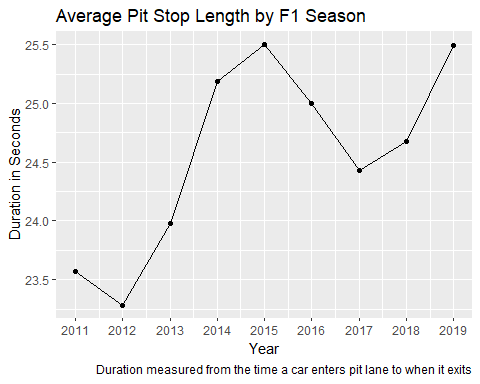
\includegraphics{part_1_files/figure-latex/unnamed-chunk-9-1.pdf}

From this graph, it appears that the variance from season to season is
minimal and unlikely to be a reason for changes in fan ratings.


\end{document}
